\section{Implementing a prototypical micro-frontend architecture}

For the evaluation of the research questions, a prototypical micro-frontend architecture was implemented. The architecture was developed in a way that it lays the ground work for being used in a production environment later. The micro-frontends are integrated using client-side integration more precisely run-time integration. The integration strategy was implemented with Webpack's Module Federation, which was described in great detail section \ref{subsection:background:micro-frontend:module-federation}. The main part of the implementation is written in Angular, but to showcase the technology agnosticism of the architecture, one micro-frontend was implemented in React. The prototype contains a single shell-application that loads all other micro-frontends. The architecture is divided into nine widgets that display only simple data and four complex single-page applications. The four SPA's are Dashboard, Contact, Sales and User.

\bigskip

\noindent @nwrl/nx is used for managing multiple micro-frontends and libraries. The key feature of Nx is the support for monorepos, which is the perfect match for micro-frontend applications. It offers support for almost any frontend framework and can be customized by plugins. Multiple related projects can be managed in a single workspace. Additionally it helps that every project uses the same version of a dependency across the workspace. Additionally Nx offers helper-functions for working with Module Federation in micro-frontends. \cite{misc::applied-methods:intro-to-nx}

\bigskip

\noindent A rough overview of the architecture is shown in figure \ref{fig:applied-methods:ui-dashboard-architecture}. It also shows a wireframe, how the application looks like. The icons inside the squares represent the JavaScript Framework used. Each widget is a separate application, that exposes a module through Module Federation, which are consumed by the Dashboard micro-frontend.

\ifshowImages
\begin{figure}[H]
    \centering
    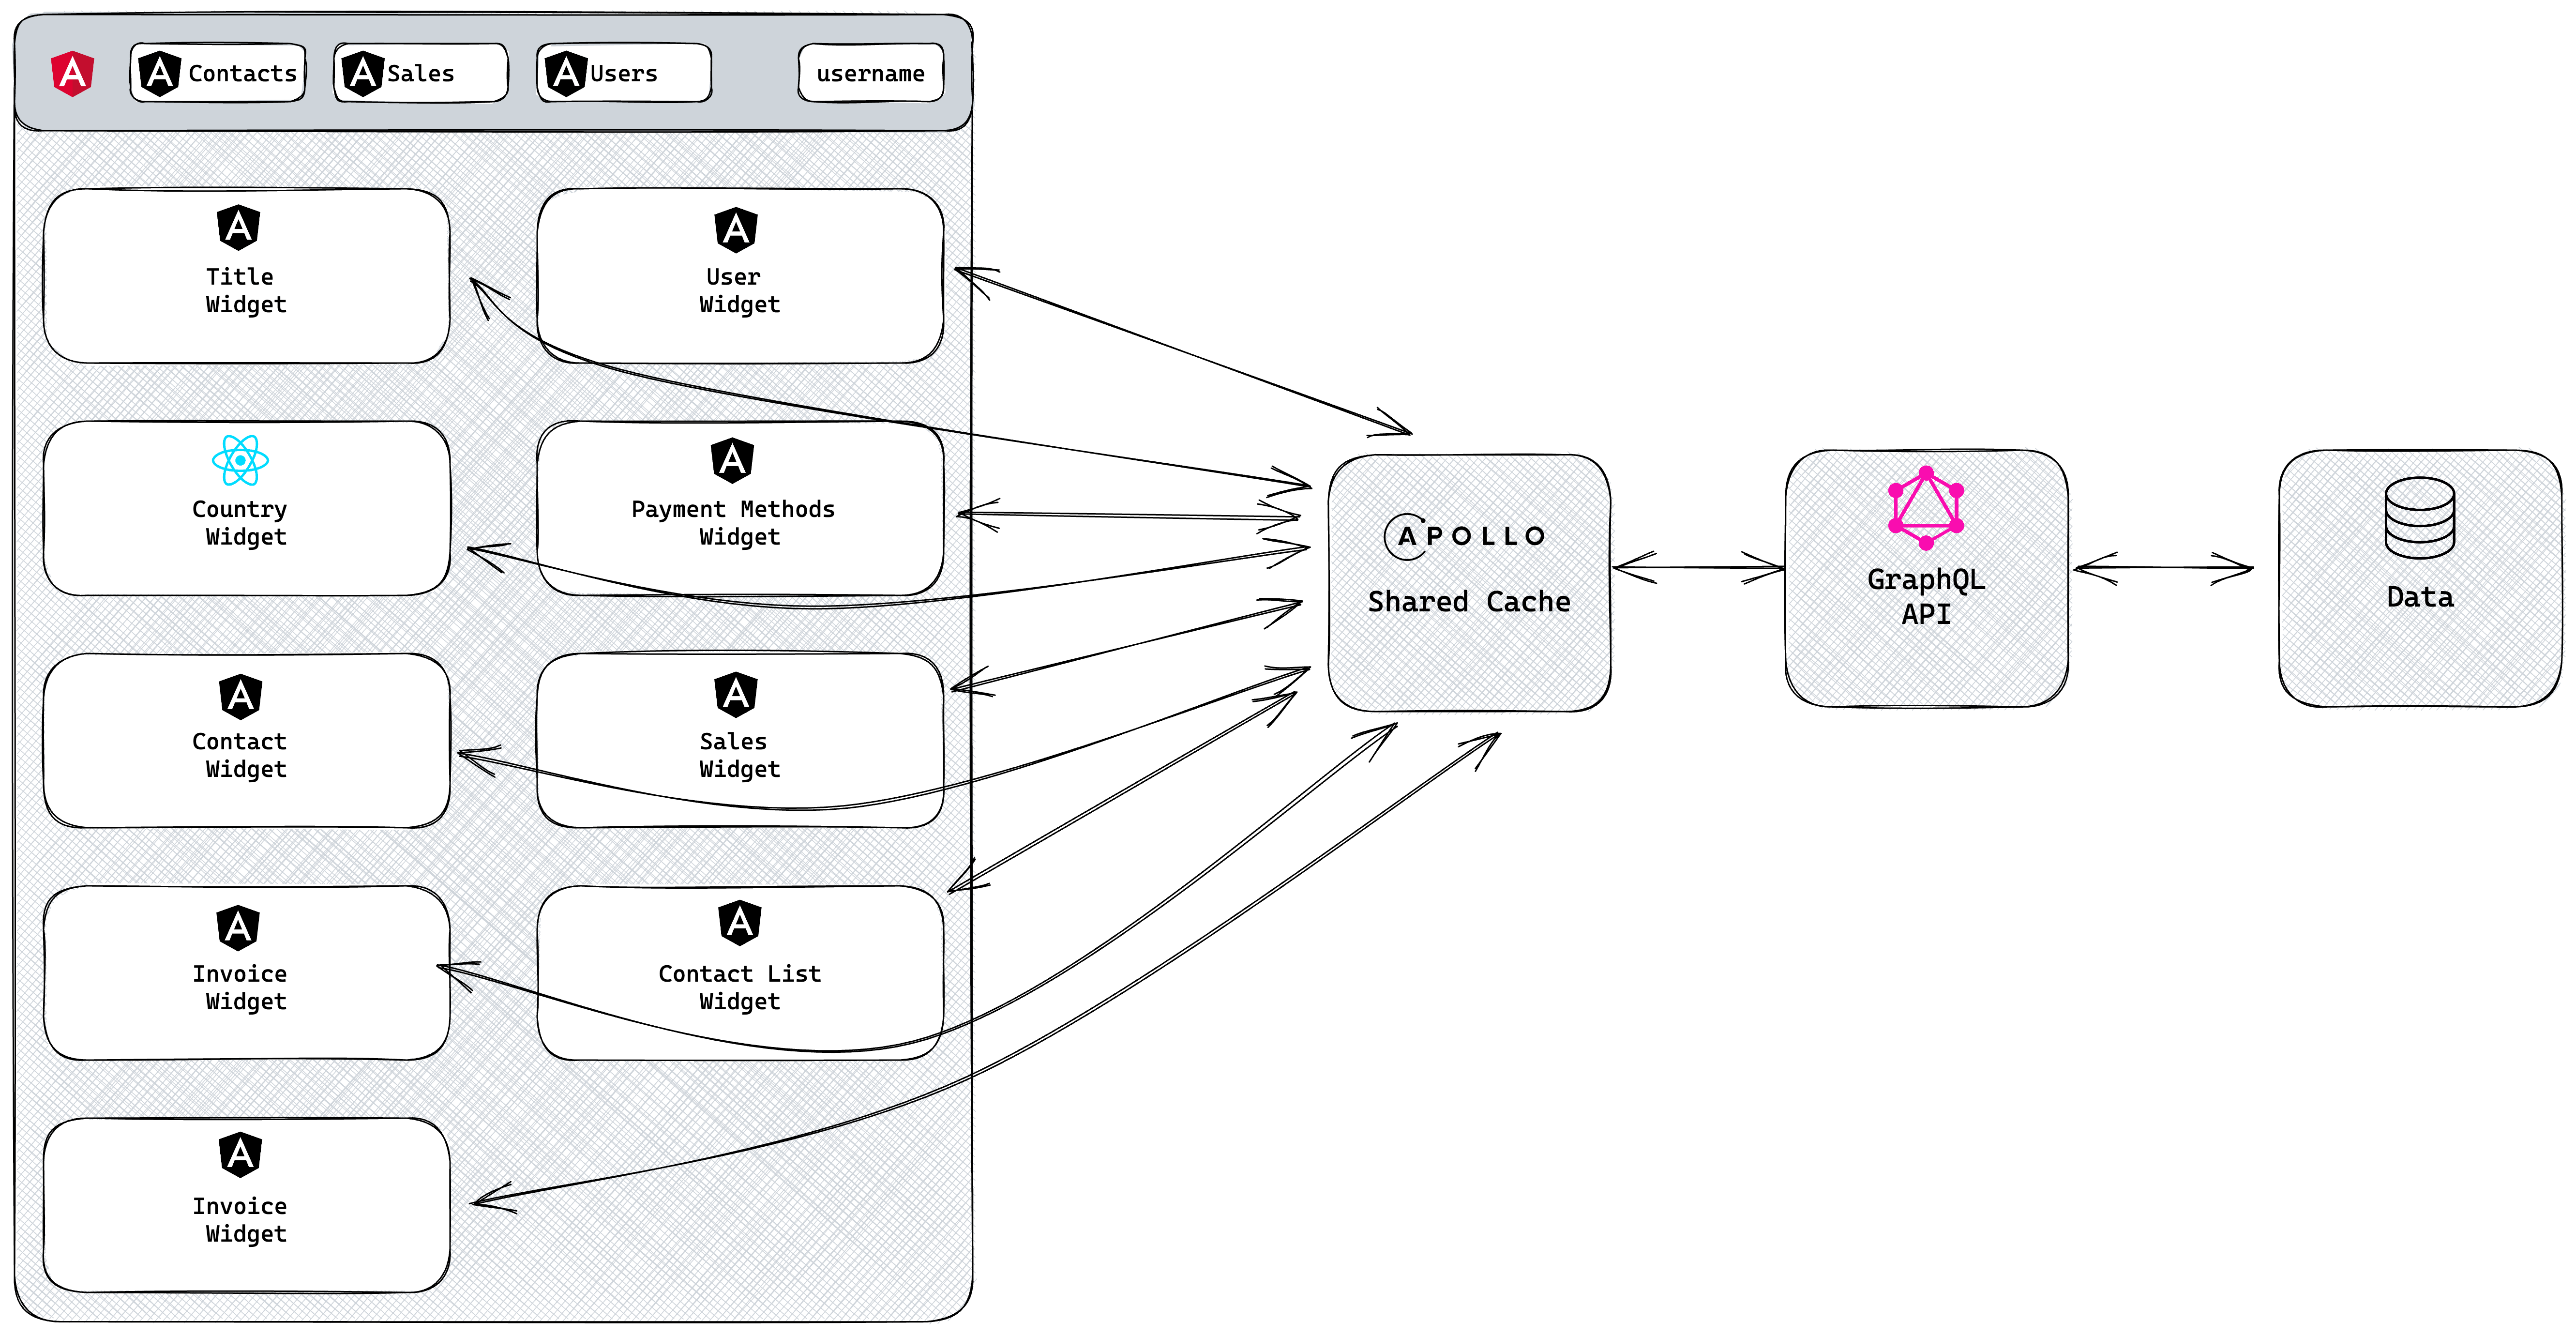
\includegraphics[width=1\linewidth]{images/ui-dashboard-architecture.png}
    \caption{Architecture of the micro-frontend prototype.}\label{fig:applied-methods:ui-dashboard-architecture}
\end{figure}
\fi

\noindent Each micro-frontend is deployed separately and is accessible by a unique URL. The application-shell is the entry point for the user. It consumes the Dashboard, Contact, Sales and User application. The main functionality of the micro-frontends are implemented in modules. This modules can be easily exposed through Module Federation and can therefore be consumed by the application-shell and by the standalone applications.

\bigskip

\noindent The listing \ref{code:methods:module-federation-config-expose} shows the configuration of the contact micro-frontend to expose its main implementation through module-federation in the form of the entry.module. The configuration of the other micro-frontends looks similar. The properties of the module-federation plugin were already discussed in section \ref{subsection:background:micro-frontend:module-federation} I define all angular- and apollo-dependencies to be shared across all micro-frontends. This is done to ensure that all micro-frontends use the same version of the dependencies. In the listing \ref{code:methods:module-federation-config-expose} the versions of the dependencies are written out. Inside the application the versions are read from the package.json to ensure consistency. The versions are also important later to ensure that the caching layer works correctly.

\ifshowListings
\begin{listing}[H]
    \begin{minted}{typescript}
module.exports = {
  name: 'contact',
  exposes: {
    './Module': 'apps/contact/src/app/remote-entry/entry.module.ts',
  },
  shared: [
    '@angular/core': {
      singleton: true, strictVersion: true, requiredVersion: '^15.1.1' 
    },
    ...
    'apollo-angular': { 
      singleton: true, strictVersion: true, requiredVersion: '^4.0.1' 
    },
    ...
  ]
};
    \end{minted}
    \caption{Module Federation config to expose the contact micro-frontend}\label{code:applied-methods:module-federation-config-expose}
\end{listing}
\fi

% TODO: explain the expose part of module federation in the module-federation section and the properties

\noindent The application shell can be configured to consume the remote-modules listed inside the remotes-object. The configuration to consume the four micro-frontends of the architecture can be seen in the listing \ref{code:methods:module-federation-config-consume}. With this configuration the application-shell consumes the entry.module.ts of the remote applications, which were exposed with the configuration from listing \ref{code:methods:module-federation-config-expose}. Just like in the configuration of the remote-modules, the application-shell has to share all dependencies as well. This is needed, so that the micro-frontends can load their runtime-dependencies from the application-shell and all use the same version.

\ifshowListings
\begin{listing}[H]
    \begin{minted}{typescript}
module.exports = {
  name: 'host',
  remotes: {
    contact: 'contact@http://localhost:4201/remoteEntry.js'
    sales: 'sales@http://localhost:4202/remoteEntry.js'
    dashboard: 'dashboard@http://localhost:4203/remoteEntry.js'
    user: 'user@http://localhost:4204/remoteEntry.js'
    'react-widget': 'dashboard-react@http://localhost:4299/remoteEntry.js'
  },
  shared: {
    '@angular/core': {
      singleton: true, strictVersion: true, requiredVersion: '^15.1.1' 
    },
    ...
    'apollo-angular': { 
      singleton: true, strictVersion: true, requiredVersion: '^4.0.1' 
    },
    ...
  }
};
    \end{minted}
    \caption{The configuration for the application-shell to consume the micro-frontends.}\label{code:applied-methods:module-federation-config-consume}
\end{listing}
\fi

\noindent With the help of the Module Federation configuration, the application-shell can load the remote modules. The remote modules are loaded asynchronously and can be referenced by the host application. The listing \ref{code:applied-methods:angular-route-to-remote-module} shows the configuration of the route to the contact micro-frontend using the Angular router. @Nwrl/nx offers helper methods like 'loadRemoteModule' for micro-frontends to load remote-modules into the routes of the application-shell. The prototype of the application-shell shows one micro-frontend per route.

\ifshowListings
\begin{listing}[H]
    \begin{minted}{typescript}
const routes: Routes = [
  {
    path: 'contact',
    loadChildren: () =>
    loadRemoteModule(
      'contact',
      './Module'
    ).then((m) => m.UiContactRemoteEntryModule),
  },
  ...
]
    \end{minted}
    \caption{Route to the contact micro-frontend.}\label{code:applied-methods:angular-route-to-remote-module}
\end{listing}
\fi

\subsection{Implement and integrate the React micro-frontend}

One widget for the dashboard micro-frontend was implemented using the popular frontend framework React. The implementation of one micro-frontend in another technology was made to show that the concept of sharing a single cache-instance between multiple micro-frontends is technology agnostic. The React widget exposes its functionality through Module Federation just like the Angular counterparts. In comparison to Angular, React does not have the concept of modules. Therefore, functionality of the widget is exported as a simple React functional component, like shown in listing \ref{code:applied-methods:module-federation-react-config-expose}.

\ifshowListings
\begin{listing}[H]
    \begin{minted}{typescript}
module.exports = {
  name: 'react-dashboard',
  exposes: {
    './Module': './src/remote-entry.ts',
  },
  shared: [
    react: {
      singleton: true, strictVersion: true, requiredVersion: '^18.2.0' 
    },
    ...
  ]
};
    \end{minted}
    \caption{Module Federation config for the React micro-frontend}\label{code:applied-methods:module-federation-react-config-expose}
\end{listing}
\fi

\noindent The host application can consume the React application in the same way as the Angular remote modules. But it is not natively possible to render a React component in an Angular application. Therefore, a wrapper Angular component was created that loads the React remote bundle and renders it inside an HTMLElement. The Angular adapter makes it possible that the Angular router points to the component, which is not possible with the React component. 
Angular modules that are consumed through Module Federation are able to access the dependency injection tree from the application-shell. But React does not offer a dependency injection system like Angular and isn't able to access the necessary dependencies. React has the concept of contexts to pass down data through the component tree, without having to pass properties down manually. It enables to share data between components that are not directly connected in the component tree. To make the shared caching layer work, the React widget needs the instance of the InMemoryCache from the application-shell. The shared caching layer is explained in section \ref{section:applied-methods:shared-caching-layer} in more detail, but the general concept is needed to understand the need of incorporating the instance into the React context. Therefore, the Angular wrapper creates the exposed widget inside a React context provider with the necessary dependencies. The function in listing \ref{code:applied-methods:prototypical-implementation:render-react-component-with-context} shows the creation of the React context provider and the rendering of the React component. 

\ifshowListings
\begin{listing}[H]
    \begin{minted}{typescript}
render<Comp extends ElementType>(rootEl: Root, Comp: Comp) {
  rootEl.render(
    createElement(
      UiNgReactContext, {
        ctx: {
          graphQLClientCache: this.inj.get(UI_GRAPHQL_CLIENT_CACHE),
          ...
        },
      },
      createElement(Comp, compProps)
    )
  );
}
    \end{minted}
    \caption{The function to render the React widget into an Angular component.}\label{code:applied-methods:prototypical-implementation:render-react-component-with-context}
\end{listing}
\fi

\noindent With the help of the function, the widget can access the instance of the InMemoryCache from the application-shell and use it to share the cache between the Angular and the React micro-frontend. How the InMemoryCache from the application-shell is injected and consumed is shown in listing \ref{code:applied-methods:prototypical-implementation:consume-react-context}. The cache is used to create a new instance of the ApolloClient and afterwards the client is provided to the application using another context.

\ifshowListings
\begin{listing}[H]
    \begin{minted}{typescript}
const injector = useContext(InjectorCtx);

const client = new ApolloClient({
  uri: injector.graphQLEndpoint,
  cache: injector.graphQLClientCache,
  ...
});

return (
  <ApolloProvider client={client}>
    <PaymentMethodList />
  </ApolloProvider>
);

    \end{minted}
    \caption{Use the InMemoryCache instance from the context.}\label{code:applied-methods:prototypical-implementation:consume-react-context}
\end{listing}
\fi

\subsection{Backend for frontend architecture}

